\documentclass[a4paper,12pt]{article}
\usepackage[left=2.5cm,right=2.5cm,top=2.5cm,bottom=2.5cm]{geometry} % Adjust page margins
\usepackage{xcolor,graphicx,framed}
\usepackage[normalem]{ulem}
\usepackage{amsmath}
\usepackage{cases}
\usepackage{gensymb}
\usepackage{chemmacros}
\setlength{\extrarowheight}{0.4cm}

\begin{document}

\newcommand{\HRule}{\rule{\linewidth}{0.4mm}} % Defines a new command for the horizontal lines, change thickness here

%----------------------------------------------------------------------------------------
%	HEADING SECTIONS
%----------------------------------------------------------------------------------------

\begin{minipage}{0.7\textwidth}
\begin{flushleft} 
\textsc{Universidad del Valle de Guatemala \\
Campus Central \\
Facultad de Ciencias y Humanidades \\
Departamento de Qu\'imica \\
Segundo ciclo, 2014 \\
Fisicoqu\'imica 1 \\
}
\end{flushleft}
\end{minipage}
~
\begin{minipage}{0.2\textwidth}
\begin{flushright}

\includegraphics[scale=0.3]{Logo_UVG} % Include a department/university logo
\end{flushright}
\end{minipage}\\

%----------------------------------------------------------------------------------------
%	TITLE SECTION
%----------------------------------------------------------------------------------------

\begin{center}
\HRule \\[0.4cm]
{ \bfseries Ejercicios en clase, 10}\\ % Title of your document
\HRule \\[0.4cm]
\end{center}

%----------------------------------------------------------------------------------------

\begin{enumerate}

 \item \textit{(Chang 6.21)} Considere el siguiente sistema en equilibrio:
$$\mbox{CaCO}_3\mbox{(s)}\;\ch{ <=> }\;\mbox{CaO(s)}+\mbox{CO}_2\mbox{(g)}$$
?`Cu\'antas fases existen? % Problema 6.21 de Chang

 \item \textit{(Chang 6.19)} Utilizar el diagrama de fases del agua para predecir la direcci\'on de los siguientes cambios:
 \begin{enumerate}
  \item en el punto triple del agua, la temperatura se reduce a presi\'on constante, y
  \item en alg\'un punto a lo largo de la curva S-L del agua, aumenta la presi\'on a temperatura constante.
 \end{enumerate} % Problema 6.19 de Chang

 \item \textit{(Chang 6.22)} En la siguiente figura se presenta un esquema aproximado del diagrama de fases del carbono. ?`Cu\'antos puntos triples tiene y cu\'ales son las fases que pueden coexistir en cada uno de ellos? ?`Cu\'al tiene mayor densidad: el grafito o el diamante? Se puede fabricar diamante sint\'etico a partir de grafito. Utilizando el diagrama de fases, ?`c\'omo har\'ia para fabricar diamante? (Ignorar la flecha en el diagrama.)
\begin{center}
 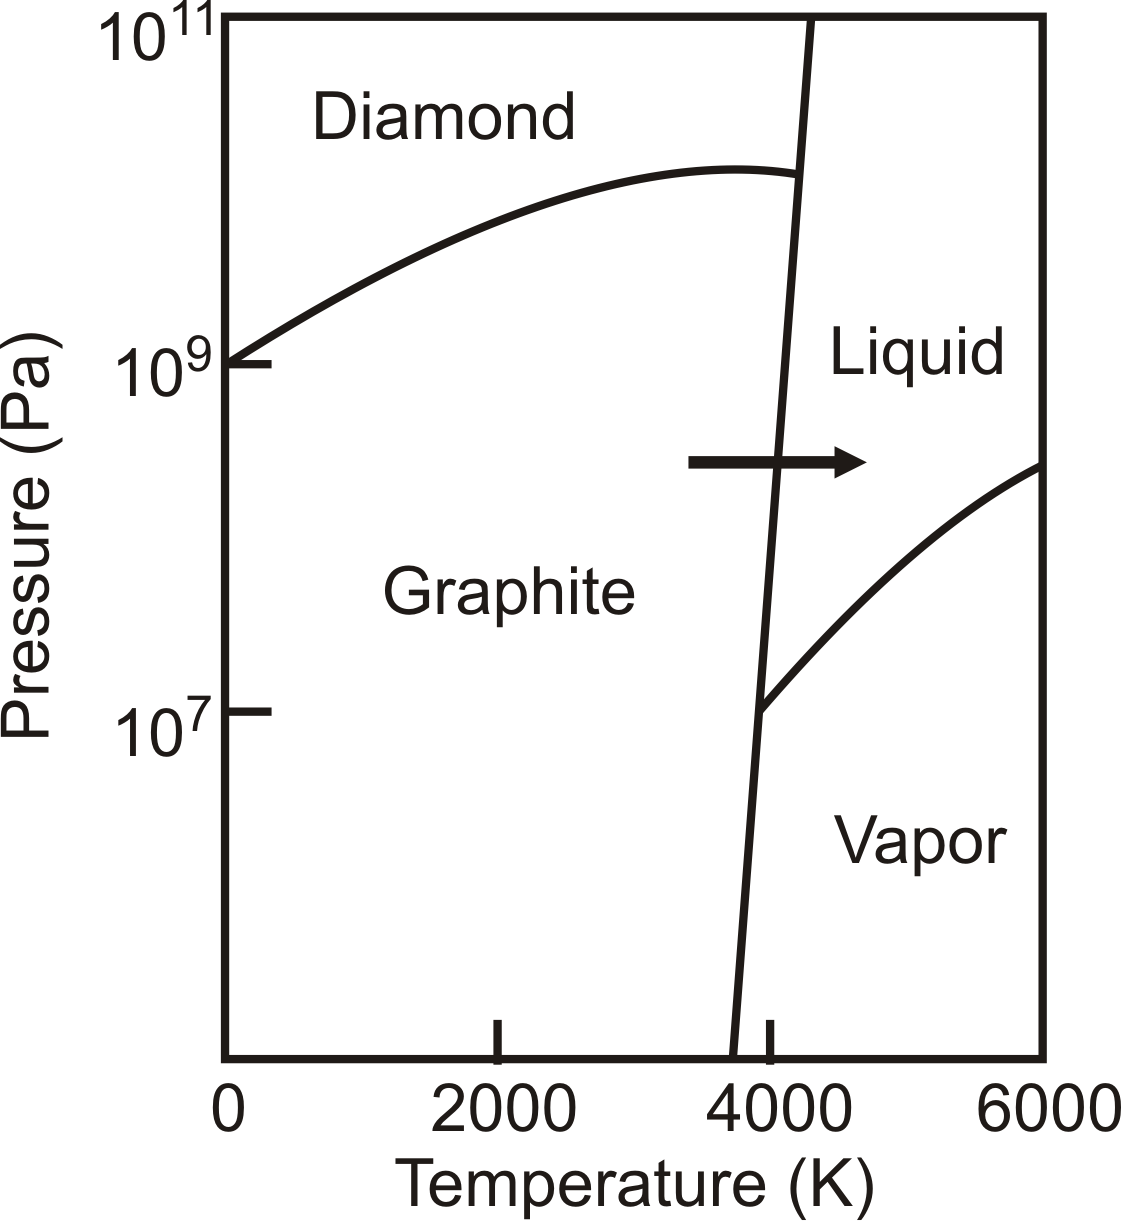
\includegraphics[scale=0.6]{figure4}
\end{center} % Problema 6.22 de Chang

 \item \textit{(McQuarrie 23-1)} Esbozar el diagrama de fase del ox\'igeno usando la siguiente informaci\'on: punto triple, $54.3\;\mbox{K}$ y $1.14\;\mbox{torr}$; punto cr\'itico, $154.6\;\mbox{K}$ y $37\,828\;\mbox{torr}$; punto de fusi\'on normal, $-218.4\celsius$; y punto de ebullici\'on normal, $-182.9\celsius$. ?`Se funde el ox\'igeno con presi\'on aplicada, de la misma forma que el agua? % Problema 9-1

 \item \textit{(McQuarrie 23-2)} Esbozar el diagrama de fase del $\mbox{I}_2$ usando la siguiente informaci\'on: punto triple, $113\celsius$ y $0.12\;\mbox{atm}$; punto cr\'itico, $512\celsius$ y $116\;\mbox{atm}$; punto de fusi\'on normal, $114\celsius$; punto de ebullici\'on normal, $184\celsius$; y la densidad del l\'iquido es mayor que la densidad del s\'olido. % Problema 9-2

 \item \textit{(McQuarrie 23-3)}  La siguiente figura muestra el diagrama de fase densidad-temperatura del benceno:
\begin{center}
 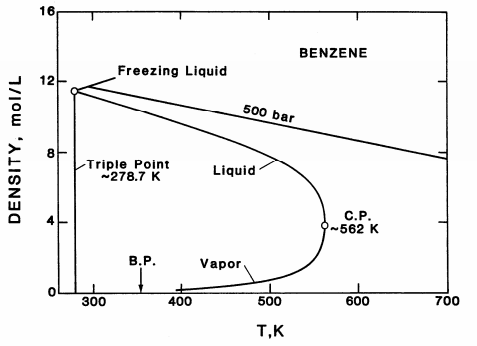
\includegraphics[scale=0.5]{figure5}
\end{center}
Usando la siguiente informaci\'on para el punto triple y el punto cr\'itico, interpretar el diagrama de fase. ?`Por qu\'e el punto triple est\'a indicado como una l\'inea en este tipo de diagrama de fase?

\begin{center}
\begin{tabular}{c|c c c c}
 &  &  & $\rho/\mbox{mol}\cdot\mbox{L}^{-1}$ & $\rho/\mbox{mol}\cdot\mbox{L}^{-1}$ \\
 & $T/\mbox{K}$ & $P/\mbox{bar}$ & Vapor & L\'iquido \\\hline
Punto triple & 278.680 & 0.04785 & 0.002074 & 11.4766 \\
Punto cr\'itico & 561.75 & 48.7575 & 3.90 & 3.90 \\
Punto de fusi\'on normal & 278.68 & 1.01325 &  &  \\
Punto de ebullici\'on normal & 353.240 & 1.01325 & 0.035687 & 10.4075  
\end{tabular}
\end{center} % Problema 9-3

 \item \textit{(McQuarrie 23-7 y 23-8)} La presi\'on de vapor del metanol a lo largo de toda la curva de co-existencia l\'iquido-vapor puede ser expresada de manera precisa por la f\'ormula emp\'irica:

\begin{center}
\begin{tabular}{r c l}
$\ln(P/\mbox{bar})$ & $=$ & $-10.752849/x+16.758207-3.603425x$\\
& & $\quad +4.373232x^2-2.381377x^3+4.572199(1-x)^{1.70}$
\end{tabular}
\end{center} 
donde $x=T/T_c$ y $T_c=512.60\;\mbox{K}$. Usar esta f\'ormula para mostrar que el punto de ebullici\'on normal del metanol es $337.67\;\mbox{K}$ y el punto de ebullici\'on est\'andar $337.33\;\mbox{K}$. % Problema 9-7 y 9-8

\end{enumerate}
 
\end{document}
